% Options for packages loaded elsewhere
\PassOptionsToPackage{unicode}{hyperref}
\PassOptionsToPackage{hyphens}{url}
\documentclass[
  ignorenonframetext,
]{beamer}
\newif\ifbibliography
\usepackage{pgfpages}
\setbeamertemplate{caption}[numbered]
\setbeamertemplate{caption label separator}{: }
\setbeamercolor{caption name}{fg=normal text.fg}
\beamertemplatenavigationsymbolsempty
% remove section numbering
\setbeamertemplate{part page}{
  \centering
  \begin{beamercolorbox}[sep=16pt,center]{part title}
    \usebeamerfont{part title}\insertpart\par
  \end{beamercolorbox}
}
\setbeamertemplate{section page}{
  \centering
  \begin{beamercolorbox}[sep=12pt,center]{section title}
    \usebeamerfont{section title}\insertsection\par
  \end{beamercolorbox}
}
\setbeamertemplate{subsection page}{
  \centering
  \begin{beamercolorbox}[sep=8pt,center]{subsection title}
    \usebeamerfont{subsection title}\insertsubsection\par
  \end{beamercolorbox}
}
% Prevent slide breaks in the middle of a paragraph
\widowpenalties 1 10000
\raggedbottom
\AtBeginPart{
  \frame{\partpage}
}
\AtBeginSection{
  \ifbibliography
  \else
    \frame{\sectionpage}
  \fi
}
\AtBeginSubsection{
  \frame{\subsectionpage}
}
\usepackage{iftex}
\ifPDFTeX
  \usepackage[T1]{fontenc}
  \usepackage[utf8]{inputenc}
  \usepackage{textcomp} % provide euro and other symbols
\else % if luatex or xetex
  \usepackage{unicode-math} % this also loads fontspec
  \defaultfontfeatures{Scale=MatchLowercase}
  \defaultfontfeatures[\rmfamily]{Ligatures=TeX,Scale=1}
\fi
\usepackage{lmodern}
\ifPDFTeX\else
  % xetex/luatex font selection
\fi
% Use upquote if available, for straight quotes in verbatim environments
\IfFileExists{upquote.sty}{\usepackage{upquote}}{}
\IfFileExists{microtype.sty}{% use microtype if available
  \usepackage[]{microtype}
  \UseMicrotypeSet[protrusion]{basicmath} % disable protrusion for tt fonts
}{}
\makeatletter
\@ifundefined{KOMAClassName}{% if non-KOMA class
  \IfFileExists{parskip.sty}{%
    \usepackage{parskip}
  }{% else
    \setlength{\parindent}{0pt}
    \setlength{\parskip}{6pt plus 2pt minus 1pt}}
}{% if KOMA class
  \KOMAoptions{parskip=half}}
\makeatother
\usepackage{longtable,booktabs,array}
\usepackage{caption}
\captionsetup[table]{skip=6pt}
\newcounter{none} % for unnumbered tables
\usepackage{calc} % for calculating minipage widths
\usepackage{caption}
% Make caption package work with longtable
\makeatletter
\def\fnum@table{\tablename~\thetable}
\makeatother
\usepackage{graphicx}
\makeatletter
\newsavebox\pandoc@box
\newcommand*\pandocbounded[1]{% scales image to fit in text height/width
  \sbox\pandoc@box{#1}%
  \Gscale@div\@tempa{\textheight}{\dimexpr\ht\pandoc@box+\dp\pandoc@box\relax}%
  \Gscale@div\@tempb{\linewidth}{\wd\pandoc@box}%
  \ifdim\@tempb\p@<\@tempa\p@\let\@tempa\@tempb\fi% select the smaller of both
  \ifdim\@tempa\p@<\p@\scalebox{\@tempa}{\usebox\pandoc@box}%
  \else\usebox{\pandoc@box}%
  \fi%
}
% Set default figure placement to htbp
\def\fps@figure{htbp}
\makeatother
\setlength{\emergencystretch}{3em} % prevent overfull lines
\providecommand{\tightlist}{%
  \setlength{\itemsep}{0pt}\setlength{\parskip}{0pt}}
% Auto-generated by infrastructure/rendering/_pdf_latex_helpers.py::extract_math_font_preamble.
% Minimal header passed to Pandoc via -H so Beamer slides pick up the same math font
% as the combined-PDF path. Adjust the manuscript's preamble.md to change the font globally.
\usepackage{unicode-math}
\setmathfont{latinmodern-math.otf}

% Slide layout defaults for warning-clean scientific decks.
\usepackage{etoolbox}
\IfFileExists{xurl.sty}{\usepackage{xurl}}{}
\IfFileExists{seqsplit.sty}{\usepackage{seqsplit}}{\newcommand{\seqsplit}[1]{#1}}
\protected\def\breakseq#1{\seqsplit{#1}}
\protected\def\breaktt#1{\begingroup\ttfamily\seqsplit{#1}\endgroup}
\setlength{\emergencystretch}{6em}
\tolerance=5000
\hbadness=10000
\hfuzz=1pt
\setlength{\tabcolsep}{2pt}
\AtBeginEnvironment{longtable}{\tiny\renewcommand{\arraystretch}{0.86}\setlength{\tabcolsep}{1pt}}
\AtBeginEnvironment{tabular}{\tiny\renewcommand{\arraystretch}{0.86}\setlength{\tabcolsep}{1pt}}
\AtBeginEnvironment{equation}{\tiny}
\AtBeginEnvironment{equation*}{\tiny}
\AtBeginEnvironment{align}{\tiny}
\AtBeginEnvironment{align*}{\tiny}
\AtBeginEnvironment{itemize}{\footnotesize}
\AtBeginEnvironment{enumerate}{\footnotesize}
\AtBeginEnvironment{description}{\footnotesize}
\setbeamerfont{caption}{size=\tiny}
\setbeamerfont{caption name}{size=\tiny}
\setbeamerfont{normal text}{size=\small}
\setbeamerfont{frametitle}{size=\small}
\setbeamerfont{section title}{size=\footnotesize}
\setbeamerfont{subsection title}{size=\footnotesize}
\setbeamertemplate{section page}{%
  \centering
  \begin{beamercolorbox}[sep=12pt,center,wd=\paperwidth]{section title}
    \parbox{0.86\paperwidth}{\centering\usebeamerfont{section title}\insertsection\par}
  \end{beamercolorbox}
}
\setbeamertemplate{subsection page}{%
  \centering
  \begin{beamercolorbox}[sep=8pt,center,wd=\paperwidth]{subsection title}
    \parbox{0.86\paperwidth}{\centering\usebeamerfont{subsection title}\insertsubsection\par}
  \end{beamercolorbox}
}
\setlength{\abovecaptionskip}{2pt}
\setlength{\belowcaptionskip}{0pt}

% Natbib and cross-reference fallbacks — slides don't load natbib
% or cleveref, but combined-PDF manuscript prose may emit these
% commands. The fallback renders citations as a bracketed key list
% and cross-references as detokenized labels so slides don't fail on
% undefined control sequences or raw underscores. \providecommand is
% a no-op if packages load later.
\providecommand{\citep}[1]{[#1]}
\providecommand{\citet}[1]{#1}
\providecommand{\citealp}[1]{#1}
\providecommand{\citeauthor}[1]{#1}
\providecommand{\citeyear}[1]{#1}
\providecommand{\cref}[1]{\texttt{\detokenize{#1}}}
\providecommand{\Cref}[1]{\texttt{\detokenize{#1}}}

% Pandoc's article template uses codelisting floats for captioned code; Beamer has no such float, so provide a slide-safe numbered block.
\newcounter{codelisting}
\renewcommand{\thecodelisting}{\arabic{codelisting}}
\newenvironment{codelisting}{%
  \refstepcounter{codelisting}%
  \begin{center}\begin{minipage}{0.96\linewidth}\footnotesize%
  \renewcommand{\caption}[1]{\par\smallskip\textbf{Listing~\thecodelisting: }##1\par\smallskip}%
}{%
  \end{minipage}\end{center}%
}
\newtheorem{proposition}{Proposition}
\newtheorem{hypothesis}{Hypothesis}
\usepackage{bookmark}
\IfFileExists{xurl.sty}{\usepackage{xurl}}{} % add URL line breaks if available
\urlstyle{same}
% fallback for those not using the hyperref driver hyperxmp:
\makeatletter
\@ifundefined{xmpquote}{\newcommand{\xmpquote}[1]{#1}}{}
\makeatother
\hypersetup{
  hidelinks,
  pdfcreator={LaTeX via pandoc}}

\author{\texorpdfstring{}{}}
\date{}

\begin{document}

\begin{frame}[allowframebreaks]{Language acquisition follows conjugate
Dirichlet updating}
\protect\phantomsection\label{sec:results-language}
Where the first study fused fixed beliefs in a single round, the second
asks whether a single agent can \emph{acquire} the likelihood of its
shared world at all, and how quickly it does so. The design is a
categorical source-mechanism analogue of the language-acquisition
mechanism discussed by Friston et al. (Friston et al. 2024): each
configured seed runs an agent that learns the likelihood of its shared
world by conjugate Dirichlet updates over 24 count batches, the count
update eq.~14. The recorded trajectory is
\(\mathrm{KL}(\text{true } A \,\|\, \text{learned } A)\) before each
batch --- it starts at the flat-prior maximum and declines monotonically
toward zero as the agent ``acquires the language'' of its world. The KL
here is the same divergence whose \(\alpha\to1\) Rényi limit is
established by Lemma 3
(eq.~3), so the learning curve and the recovery
\end{frame}

\begin{frame}[allowframebreaks]{Language acquisition follows conjugate
Dirichlet updating}
limits measure the same object.

\end{frame}

\begin{frame}[allowframebreaks]{Language acquisition follows conjugate
Dirichlet updating}
\begin{itemize}
\tightlist
\item
  Initial KL (flat prior): 3.4231
\item
  Final KL (after 24 batches): 0.0027
\item
  Total KL reduction: 3.4204
\item
  Trajectory points: 25 ordered learning steps per seed
\item
  Pointwise seed bootstrap: 95\% intervals over \(n = 480\) independent
  seeds
\item
  Trajectory monotone-decreasing: Yes
\end{itemize}

\end{frame}

\begin{frame}[allowframebreaks]{Language acquisition follows conjugate
Dirichlet updating}
The monotone decline to a final KL of 0.0027 is the demonstrated
quantity behind the acquisition claim: under the tested count schedule,
the learned likelihood moves toward the true generative likelihood as
conjugate counts accumulate. This finite trajectory is evidence of the
update's behavior, not a convergence-rate result for arbitrary
data-generating processes.

\end{frame}

\begin{frame}[allowframebreaks]{Language acquisition follows conjugate
Dirichlet updating}
\begin{figure}
\centering
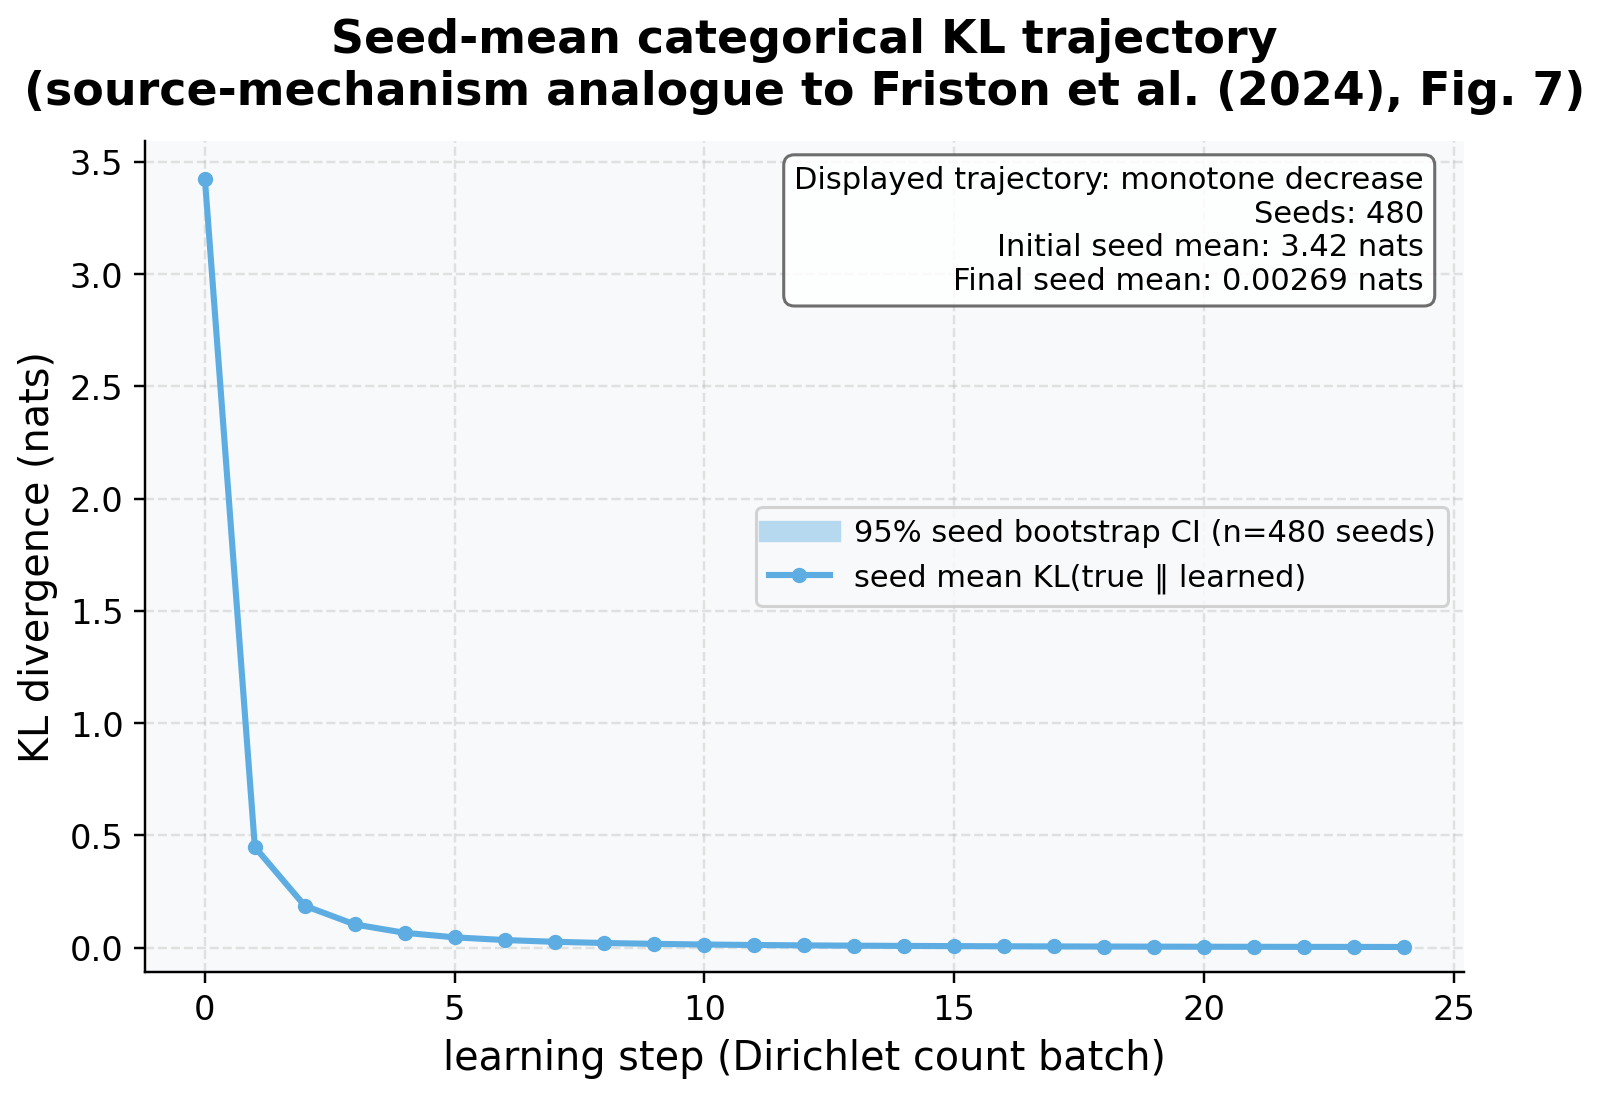
\includegraphics[width=0.8\linewidth,height=0.40\textheight,keepaspectratio,alt={Seed-mean KL divergence from the true likelihood A to the learned likelihood A. The plotted quantity is \textbackslash mathrm\{KL\}(\textbackslash text\{true \}A \textbackslash,\textbackslash\textbar\textbackslash, \textbackslash text\{learned \}A). Source relation: source-mechanism analogue to Friston et al.~(2024), Fig. 7; estimand: seed-mean KL in nats by ordered learning step. x-axis: ordered Dirichlet count batch, from the flat prior at zero through all 24 batches (25 points per seed); y-axis: summed per-column KL divergence between the true likelihood and the current expected likelihood, in nats. The solid line is the mean over 480 independent configured seeds, and the shaded band is the pointwise 95\% percentile-bootstrap interval resampling seeds at each learning step. The replication unit is seed, not the ordered trajectory points. The mean curve falls monotonically from 3.4231 nats to 0.0027 nats (total reduction 3.4204 nats, computed from the unrounded endpoints); the computed monotone-decreasing verdict is Yes. This reduced categorical protocol is related to, but does not exactly reproduce, the richer multi-episode protocol in Friston et al.~(2024).}]{../figures/language_kl_decay.png}
\caption{Seed-mean KL divergence from the true likelihood A to the
learned likelihood A. The plotted quantity is
\(\mathrm{KL}(\text{true }A \,\|\, \text{learned }A)\). Source relation:
source-mechanism analogue to Friston et al.~(2024), Fig. 7; estimand:
seed-mean KL in nats by ordered learning step. x-axis: ordered Dirichlet
count batch, from the flat prior at zero through all 24 batches (25
points per seed); y-axis: summed per-column KL divergence between the
true likelihood and the current expected likelihood, in nats. The solid
line is the mean over 480 independent configured seeds, and the shaded
band is the pointwise 95\% percentile-bootstrap interval resampling
seeds at each learning step. The replication unit is seed, not the
ordered trajectory points. The mean curve falls monotonically from
3.4231 nats to 0.0027 nats (total reduction 3.4204 nats, computed from
the unrounded endpoints); the computed monotone-decreasing verdict is
Yes. This reduced categorical protocol is related to, but does not
exactly reproduce, the richer multi-episode protocol in Friston et
al.~(2024).}\label{fig:language-kl}
\end{figure}

\end{frame}

\begin{frame}[allowframebreaks]{Language acquisition follows conjugate
Dirichlet updating}
fig.~\ref{fig:language-kl} plots the full learning curve and its CI
band.
\end{frame}

\end{document}
